\subsection{Interactions with other Services}

The main \LB\ functionality is keeping track of jobs managed by
the Workload Management System otherwise.
Therefore its basic usage is done internally by the WMS components.
However, the query and notification interface is completely available
to user-level applications. Upto limited extent (two event types)
this holds for the event-logging interface too.

\subsubsection{Event sources}
\LB\ events are generated by the following WMS components:
\begin{description}
\item[User Interface] registers the job with \LB\ and provides details
on transfer of the job to the resource broker.
\item[Resource Broker,] consisting of several WMS components,
logs various events as the job is passed among these components, 
as well as other important job-related information (\eg\ the chosen
destination Computing Element).
\item[Computing Element,] via the Job Wrapper script, provides the immediate
information on job execution.
\end{description}
Besides these WMS components the job payload may also log UserTag events
(see Sect.~\ref{log_usertag}) containing arbitrary user information.

Checkpointable jobs also use \LB\ to keep track of the job progress.
This is done internally by the checkpoint support library.

Finally, changes of job access control lists are done by logging
another event. This may be done directly by the user or using the WMS
user interface.

\subsubsection{Queries}

The \LB\ queries with a~user-visible output
are executed from within WMS User Interface
commands glite-job-status and glite-job-logging-info.

Besides those several WMS components use \LB\ internally to query
information on job status which is relevant for their processing.

\subsubsection{Notifications}

Notifications on job state change are used by WMS GUI 
to monitor the state of jobs periodically.

\subsubsection{Component and Interaction Diagrams}
% \todo{nekdy priste}
% To help understanding the service a set of component and interaction
% diagrams might help. This section is not mandatory.

\begin{figure}[h]
\centering
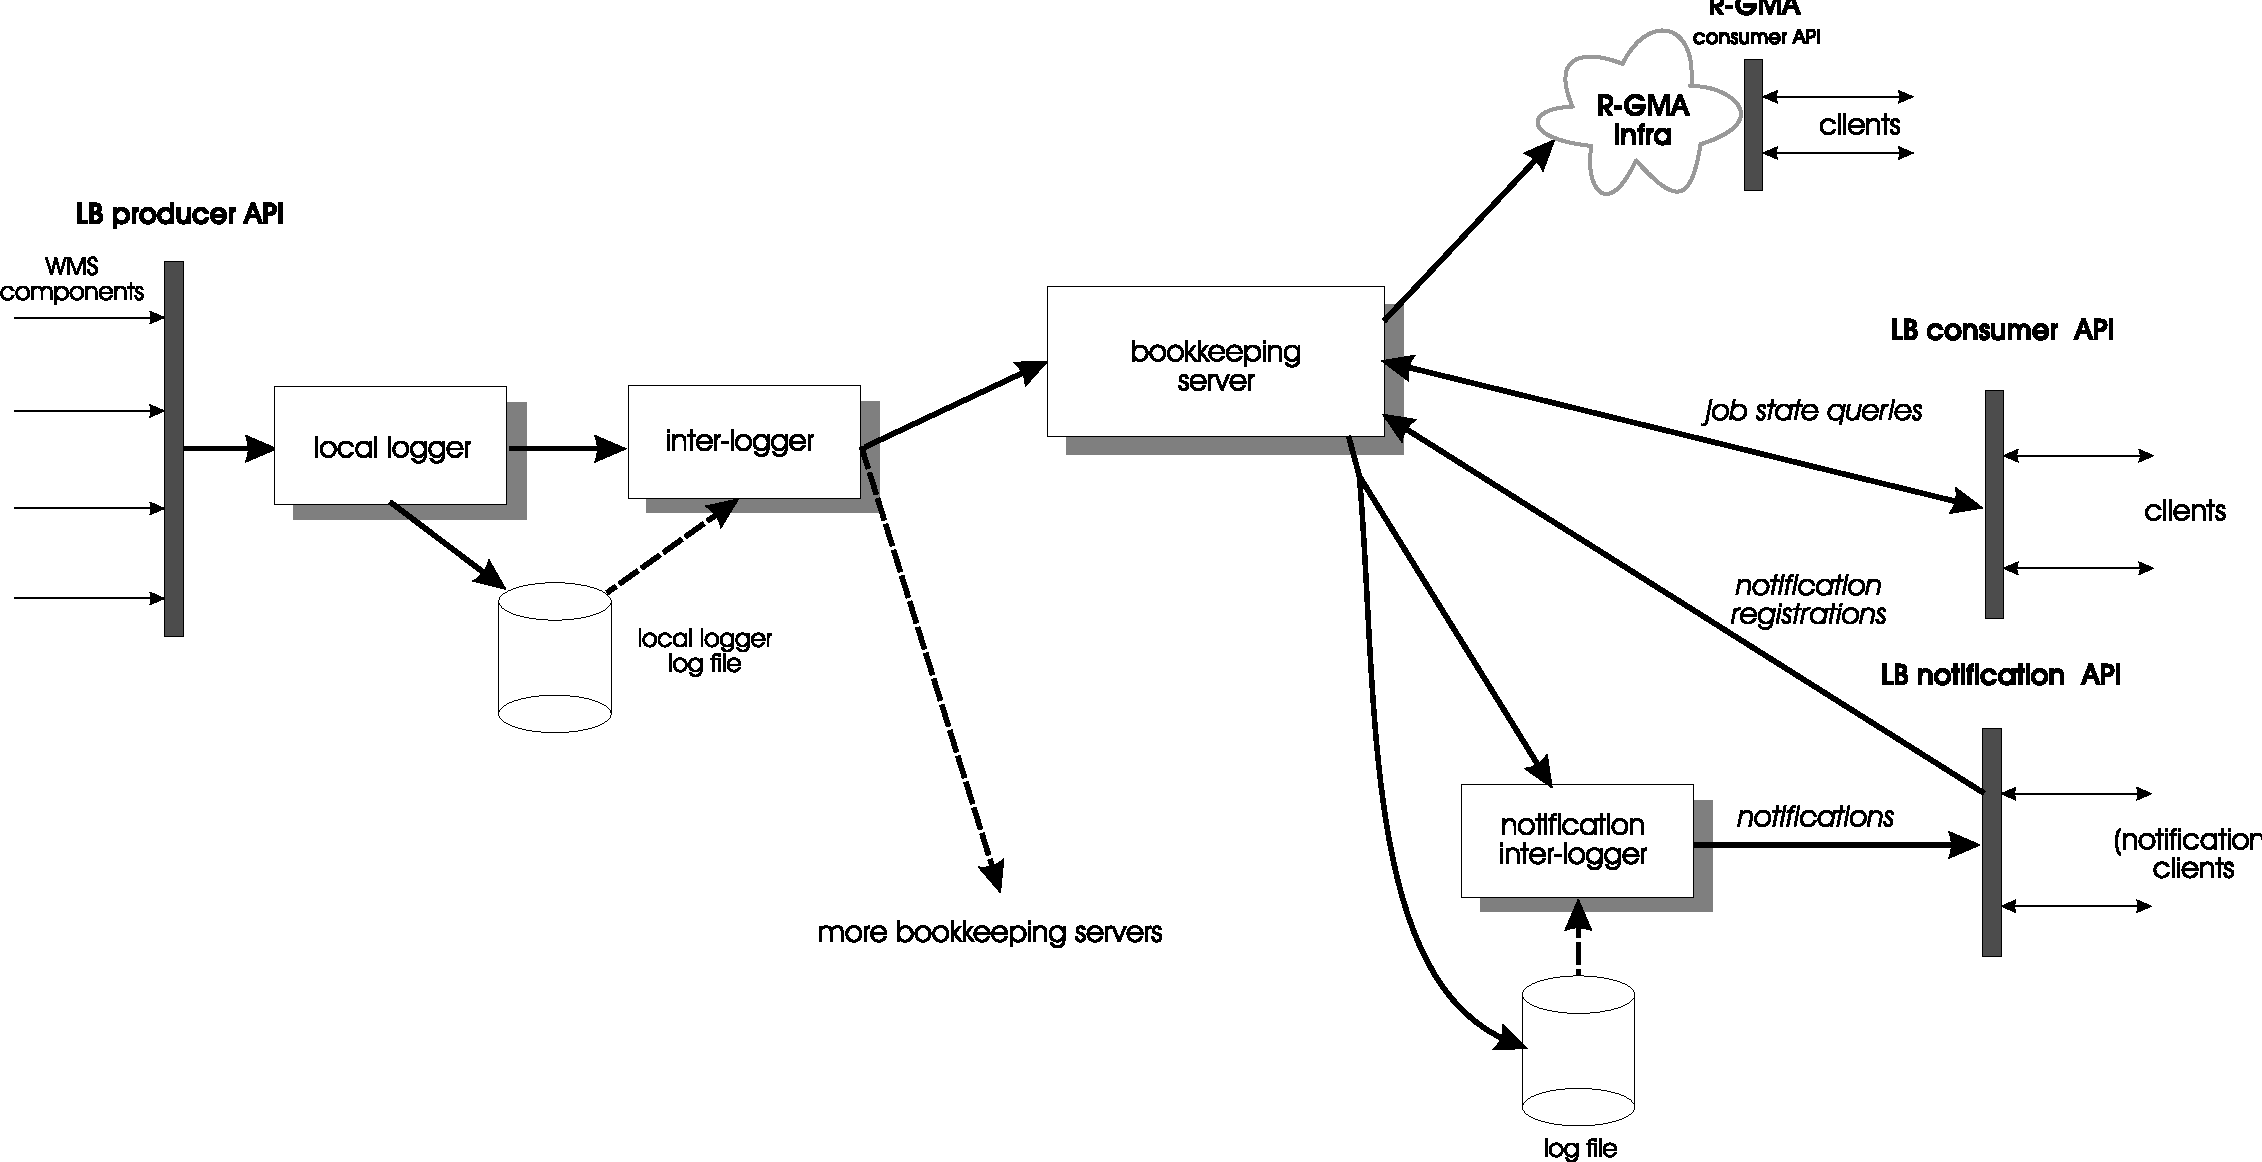
\includegraphics[width=.8\hsize]{logging-arch-notif}
\caption{Overview of the \LB\ architecture}
\label{fig-arch}
\end{figure}


\endinput
